\newpage
\subsection{UC3 - Modifica Metadati}
\label{subsec:uc3}

\begin{figure}[h]
    \centering
    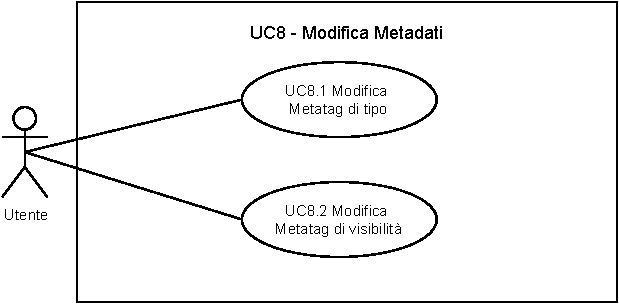
\includegraphics[width=0.7\textwidth]{componenti/casi-duso/diagrammi/UC3.pdf}
    \caption{Diagramma rappresentante UC3}
    \label{fig:UC3}
\end{figure}

\begin{itemize}
    \item \textbf{Descrizione}: L’utente vuole modificare uno o più metadati attualmente assegnati al dataset.
	
    \item \textbf{Attore primario}: Utente.
    
    \item \textbf{Precondizione}:   Nel programma è stato importato un dataset dotato di metadati per ogni sua colonna.
    \item \textbf{Postcondizione}:  Vengono aggiornati i metadati del dataset se modificati.

	\item \textbf{Scenario principale}:
        \begin{enumerate}
			\item L'utente effettua modifiche che ritiene necessarie tra quelle possibili.
			\item L'utente conferma le modifiche premendo il pulsante di salvataggio.
        \end{enumerate}

    %TODO: Riprisino è comunque un aggiornamento giusto? Dovremmo mettere un'estensione?
    \item \textbf{Scenario alternativo}:
		\begin{enumerate}
			\item L'utente decide di annullare le modifiche selezionando il pulsante "annulla".
			\item Vengono ripristinati i metatag precedenti alla modifica.
        \end{enumerate}
\end{itemize}

\newpage
\subsubsection{UC3.1 - Modifica metadati di tipo}
\label{subsubsec:uc3.1}

\begin{itemize}
    \item \textbf{Descrizione}: L’utente vuole modificare uno o più metadati di tipo attualmente assegnati alle dimensioni del dataset.
	
    \item \textbf{Attore primario}: Utente.
    
    \item \textbf{Precondizione}:   Nel programma è stato importato un dataset dotato di metadati per 
                                    ogni sua colonna e l'utene seleziona la voce di modifica dei metadati di tipo.
    \item \textbf{Postcondizione}:  Vengono aggiornati i metadati di tipo del dataset che sono stati modificati.

	\item \textbf{Scenario principale}:
		\begin{enumerate}
            \item L'utente seleziona le dimensioni del dataset che vuole modificare.
            \item L'utente modifica il metadato di tipo di ogni dimensione selezionata tra le opzioni possibili.
        \end{enumerate}
\end{itemize}


\subsubsection{UC3.2 - Modifica metadati di visibilità}
\label{subsubsec:uc3.2}

\begin{itemize}
    \item \textbf{Descrizione}: L’utente vuole modificare i metadati di visibilità attualmente assegnati al dataset.
	
    \item \textbf{Attore primario}: Utente.
    
    \item \textbf{Precondizione}:   Nel programma è stato importato un dataset dotato di metadati per 
                                    ogni sua colonna e l'utene seleziona la voce di modifica dei metadati di visibilità.
    \item \textbf{Postcondizione}:  Vengono aggiornati i metadati di visibilità del dataset che sono stati modificati.

	\item \textbf{Scenario principale}:
		\begin{enumerate}
            \item L'utente seleziona le dimensioni del dataset che vuole modificare.
            \item L'utente decide se rendere visibile o meno le dimensioni selezionate.
        \end{enumerate}
\end{itemize}

